\subsection{Función print()}
La función print() en Python es una herramienta fundamental para mostrar información en la consola o en la salida estándar del programa. Su propósito principal es facilitar a lo programadores imprimir mensajes, variables, listas y otros datos que permiten observar el comportamiento del código.

\begin{itemize}
    \item Salida de texto: print() Se utiliza para mostrar cadenas de textos en la consola. Esto se útil para comunicar mensajes, indicadores o información relevante durante la ejecución del programa.
    \begin{figure}[h]
        \centering
        \scalebox{0.35}{
        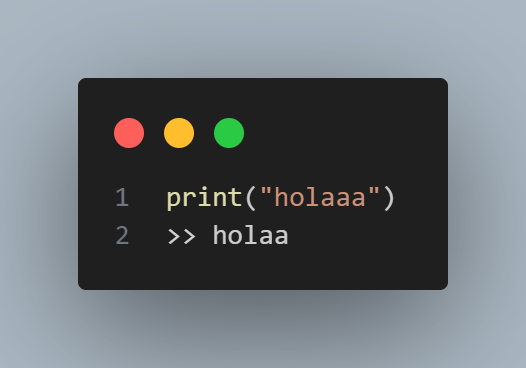
\includegraphics{Imagenes/entrada1.png}
        }
      \end{figure}

    \item Imprimir variables: Imprimir variables es una práctica común en programación, ya que te permite observar el contenido de las variables en diferentes momentos de la ejecución de tu programa. Esto es esencial para el seguimiento del flujo de datos en tu código, a continuación se muestran algunos ejemplos.
\begin{itemize}
    
    \item Ejemplo 1 : Para imprimir el valor de una variable, simplemente incluye a la variable como argumento de la función.
    \begin{figure}[h]
        \centering
        \scalebox{0.35}{
        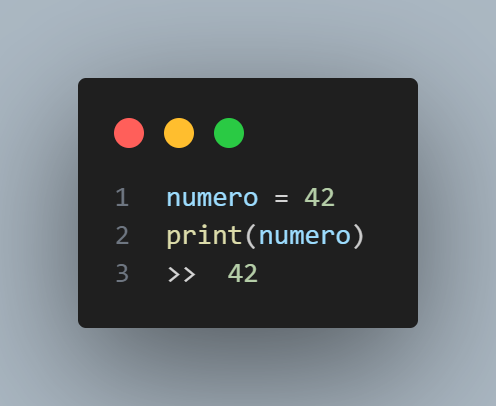
\includegraphics{Imagenes/entrada2.png}
        }
      \end{figure}

    \item Ejemplo 2 : Concatenar variables de texto. Puedes combinar el valor de una variable con texto utilizando el operador de concatenación(+). esto es útil para crear mensajes informativos
    \begin{figure}[h]
        \centering
        \scalebox{0.35}{
        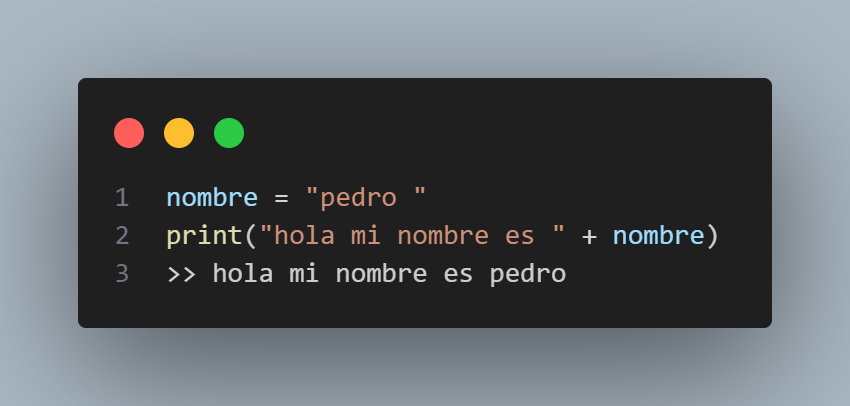
\includegraphics{Imagenes/entrada3.png}
        }
      \end{figure}
\end{itemize}   
\end{itemize}

\subsection{Función input()}
Ahora cómo enviar un dato mediante el teclado para que el programa lo tome en cuenta mediante el método input()

\begin{itemize}
    \item Ejemplo 1
    \begin{figure}[h]
        \centering
        \scalebox{0.35}{
        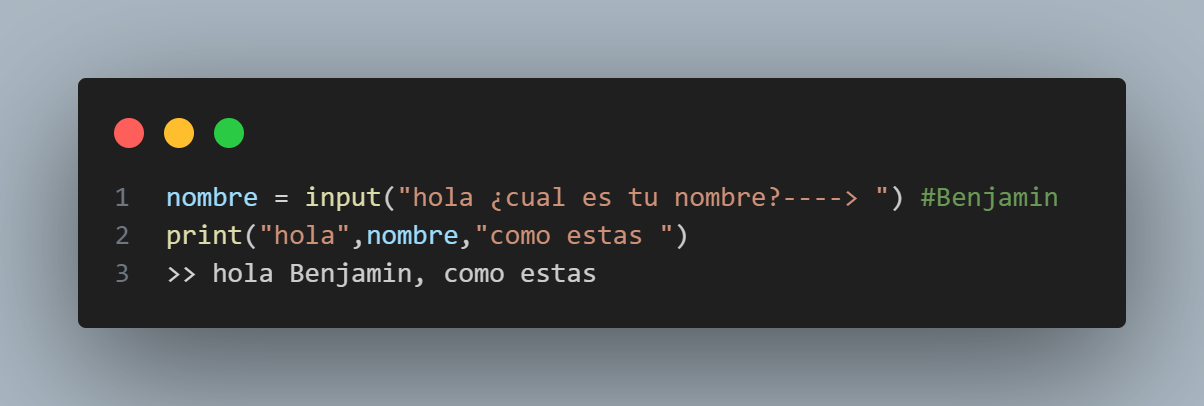
\includegraphics{Imagenes/entrada4.png}
        }
      \end{figure}
\end{itemize}

Esta función permite obtener el texto escrito por el usuario, al cual se le asignará un espacio a la memoria con la variable que el programador crea conveniente. Al llegar a la línea del comando, la consola esperara respuesta.Cuando el usuario escriba algo y presione la tecla Enter, el código seguirá ejecutándose.\\

Lo que estamos indicando al programa es que la variable «nombre» va a tomar el valor que el usuario ingrese cuando se le muestre el mensaje «Hola ¿Cuál es tu nombre?», para posteriormente, responder con otro mensaje y el valor que se ingresó. Debemos tener en cuenta que al usar input(), los datos ingresados siempre serán guardados como tipo string. Si necesitáramos ingresar números para utilizarlos en alguna operación matemática, debemos convertirlos a un tipo de dato adecuado (por ejemplo int o float, dependiendo si requerimos decimales). Podemos hacerlo de las siguientes maneras

\begin{figure}[h]
    \centering
    \scalebox{0.35}{
    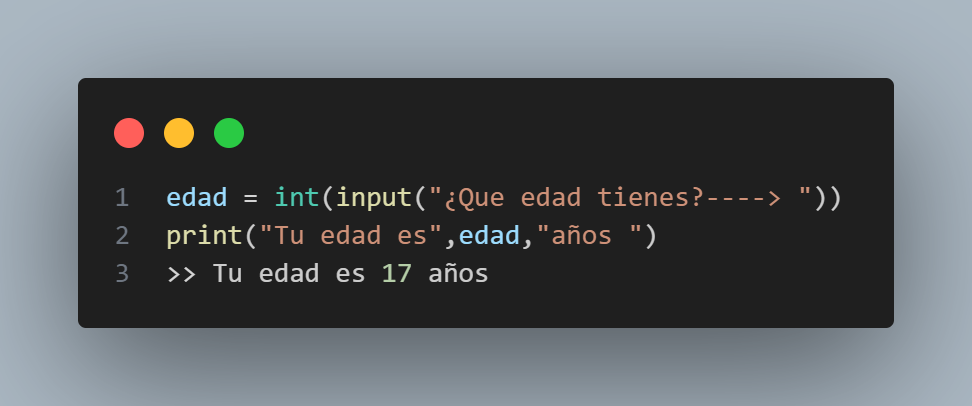
\includegraphics{Imagenes/entrada5.png}
    }
  \end{figure}

\subsection{Formateo de cadenas}

Python ofrece varias formas de formatear cadenas,y dos de los más comunes son mediantes f-strings(cadenas formateadas) y métodos de formatos.
\begin{itemize}
    \item Utilizan la sintaxis de cadenas con una “f” o “F” 
    \item Permiten incrustar expresiones o variables mediante llaves ``{}''
    \item Pueden realizar cambios y formateos dentro de la llave.
    \item Son una forma más legibles y eficiente de formatear cadenas en python.
\end{itemize}

En python, una cadena de texto normal se escribe entre comillas (``''), para crear f-strings solo tienes que agregar la letra f o F mayúscula antes de la comilla.\\

\newpage
¿Cómo imprimir variables usando f-strings?

\begin{figure}[h]
    \centering
    \scalebox{0.35}{
    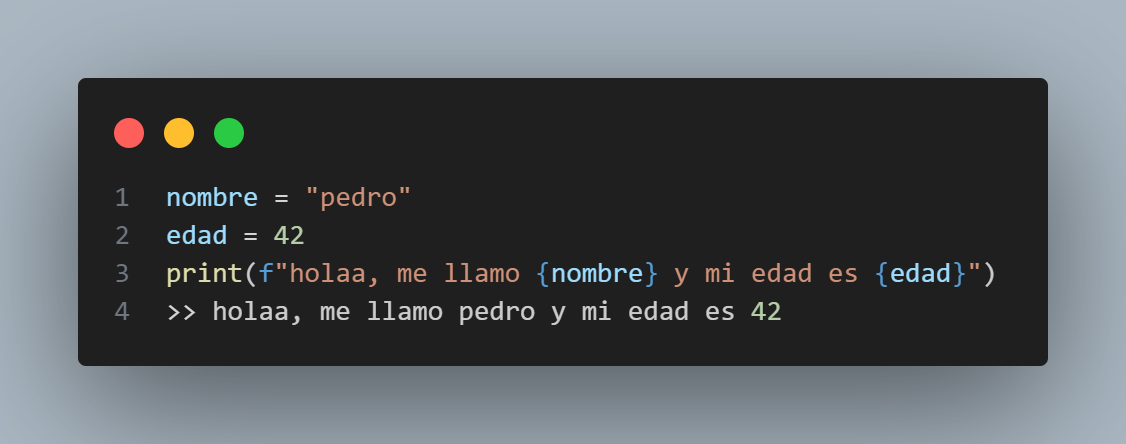
\includegraphics{Imagenes/entrada6.png}
    }
  \end{figure}

¿Cómo evaluar expresiones en python con f-string?\\

Como las f-Strings son evaluadas al momento de ejecución (cuando se está ejecutando el código Python), bien podrías usar una f-string para evaluar expresiones válidas.\\

En el siguiente ejemplo. num1 y num2 son nuestras variables, para obtener el producto de estas variables únicamente basta con escribir la siguiente expresión num1 * num2 dentro de llaves
\begin{figure}[h]
    \centering
    \scalebox{0.35}{
    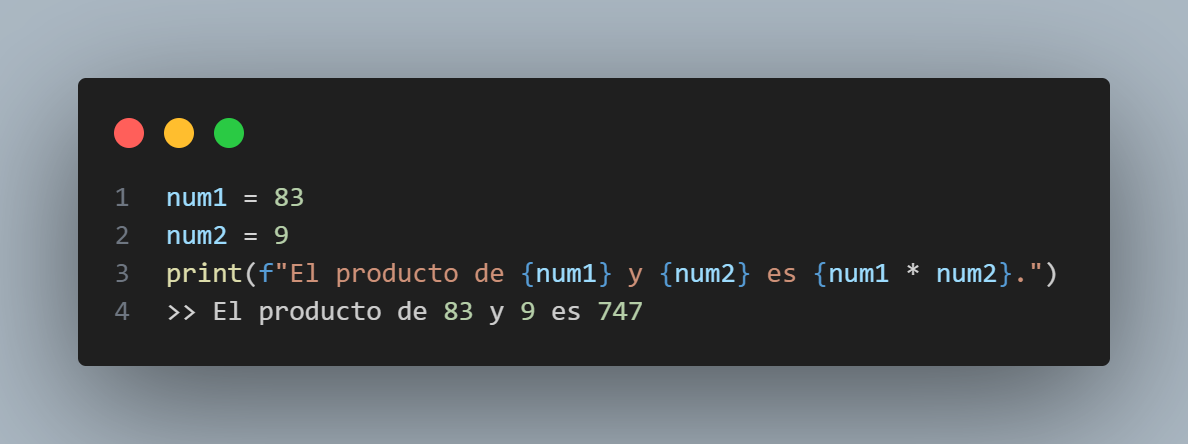
\includegraphics{Imagenes/entrada7.png}
    }
  \end{figure}

En cualquier f-string,  {variable nombre} y {expresión} se sustituirán  por los valores que representan  o por el valor resultante de una operación en el momento de ejecución (cuando se está ejecutando el código Python)
